
\begin{enumerate}

\item The polyhedron is represented in  Figure~\ref{fig:poly}

  \begin{figure}[htb]
  \begin{center}
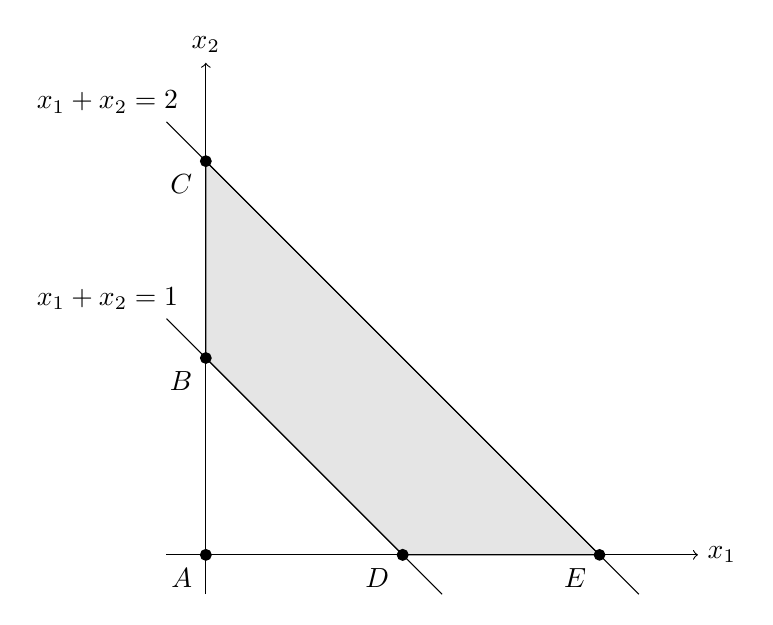
\begin{tikzpicture}[scale = 2.5]
\draw[fill=gray!20]  (1,0) -- (2,0) -- (0,2) -- (0,1) -- (1,0) -- cycle;
\draw[->] (-0.2,0) -- (2.5,0) node[right] {$x_1$};
\draw[->] (0,-0.2) -- (0,2.5) node[above] {$x_2$};
\draw (-0.2,2.2) -- (2.2,-0.2);
\node at (-0.5,2.3) {$x_1 + x_2 = 2$};
\draw (-0.2,1.2) -- (1.2,-0.2);
\node at (-0.5,1.3) {$x_1 + x_2 = 1$};
\node [circle,fill=black,draw,scale=0.2,label=below left:$A$] at (0,0) {A};
\node [circle,fill=black,draw,scale=0.2,label=below left:$B$] at (0,1) {B};
\node [circle,fill=black,draw,scale=0.2,label=below left:$C$] at (0,2) {C};
\node [circle,fill=black,draw,scale=0.2,label=below left:$D$] at (1,0) {D};
\node [circle,fill=black,draw,scale=0.2,label=below left:$E$] at (2,0) {E};

\end{tikzpicture}
  \end{center}
  \caption{\label{fig:poly}The constraint polyhedron}
  \end{figure}
  Note that it has four vertices, labeled B, C, D and E.
  
\item
The polyhedron can be written in standard form by introducing non
negative slack variables, and rewriting the constraints in the form of equality constraints:

\begin{align*}
-x_1-x_2+x_3 & =-1,\\
x_1+x_2+x_4 &=2,\\
x_1,x_2,x_3,x_4 & \geq 0.
\end{align*}

The equality constraints in matrix form are
\[
Ax= b,
\text{ where }
 A \in \mathbb{R}^{2\times 4},\; b \in \mathbb{R}^2,\; x \in \mathbb{R}^4,
\]
\[
A =
\begin{pmatrix*}[r]
-1&-1&1&0\\
1&1&0&1
\end{pmatrix*},\;
b =
\begin{pmatrix*}[r]
-1\\
2
\end{pmatrix*}.
\]

\item
This is a problem with $n=4$ variables and $m=2$ equality
constraints. Therefore, the total number of potential bases is 6. 
Let's investigate them.

\begin{enumerate}
\item $x_3$ and $x_4$ in the basis. We consider the third and fourth columns of matrix A which form the matrix $$B =
\begin{pmatrix*}[r]
1&0\\
0&1
\end{pmatrix*}.$$
It is invertible, therefore it is a valid basis. 
We set the non basic variables $x_1$ and $x_2$ to zero. Then: 
$$
x_B=B^{-1}b=
\begin{pmatrix*}[r]
-1\\
2
\end{pmatrix*};
x =
\begin{pmatrix*}[r]
0\\
0\\
-1\\
2
\end{pmatrix*}.$$
$x_B$ has a negative entry. The basic solution is not a \emph{feasible}
basic solution. Therefore, it does not correspond to a vertex of the
polyhedron. Setting $x_1$ and $x_2$ to zero corresponds to point $A=(0,0)$
in Figure~\ref{fig:poly}. At that point, two constraints are active: $x_1 \geq 0$
and $x_2 \geq 0$, as it is a basic solution. But it is clearly outside
of the polyhedron, and it is not a vertex.

\item $x_1$ and $x_3$ in the basis. We consider the first and third columns of matrix A which form the matrix $$B =
\begin{pmatrix*}[r]
-1&1\\
1&0
\end{pmatrix*}.$$
This matrix is invertible. Therefore, we have a valid basis. 
We set the non basic variables $x_2$ and $x_4$ to zero. Then: 
$$B^{-1} =
\begin{pmatrix*}[r]
0&1\\
1&1
\end{pmatrix*}
;
x_B=B^{-1}b=
\begin{pmatrix*}[r]
2\\
1
\end{pmatrix*}
;
x
=
\begin{pmatrix}
2\\
0\\
1\\
0
\end{pmatrix}.
$$
$x_B$ is non negative, and we have a feasible basic solution. It
corresponds to a vertex of the polyhedron. This is the point $E=(2,0)$
in Figure~\ref{fig:poly}. At that point, two constraints are active: $x_1+x_2
\leq 2$
and $x_2 \geq 0$. In standard form, it means that constraints $x_4
\geq 0$ and $x_2 \geq 0$ are active. It shows that setting the non
basic variables to zero is equivalent to impose the corresponding
constraints to be active. 

\item $x_1$ and $x_2$ in the basis. We consider the first and second columns of matrix A which form the matrix 
$$B = \begin{pmatrix*}[r]
-1&-1\\
1&1
\end{pmatrix*}.$$
This matrix $B$ is singular. Therefore, this is not a valid
basis. From a geometrical point of view, a basis is at the
intersection of two constraints. But, here, the non basic variables
$x_3$ and $x_4$ correspond to  two parallel
constraints. They have no intersection.

\item $x_1$ and $x_4$ in the basis. We consider the first and fourth columns of matrix A which form the matrix
$$B = \begin{pmatrix*}[r]
-1&0\\
1&1
\end{pmatrix*}.$$
  The basic matrix is invertible. It is therefore a valid basis.  
We set the non basic  variables $x_2$ and $x_3$ to zero. Then: 
$$
B^{-1} =
\begin{pmatrix*}[r]
-1&0\\
1&1
\end{pmatrix*}
;
x_B=B^{-1}b=
\begin{pmatrix*}[r]
1\\
1
\end{pmatrix*}
;
x
=
\begin{pmatrix}
1\\
0\\
0\\
1
\end{pmatrix}.
$$
$x_B$ is non negative, and we have a feasible basic solution. It
corresponds to the point $D=(1,0)$ in Figure~\ref{fig:poly}.

\item $x_2$ and $x_3$ in the basis. We consider the second and third columns of matrix A which form the matrix 
$$B = \begin{pmatrix*}[r]
-1&1\\
1&0
\end{pmatrix*}.$$
  It is invertible, and we have a valid basis. 
We set the non basic variables $x_1$ and $x_4$ to zero. Then: 
$$
B^{-1} =
\begin{pmatrix*}[r]
0&1\\
1&1
\end{pmatrix*}
;
x_B=B^{-1}b=
\begin{pmatrix*}[r]
2\\
1
\end{pmatrix*}
;
x
=
\begin{pmatrix}
0\\
2\\
1\\
0
\end{pmatrix}.
$$
It is non negative, and corresponds to the point $C=(0,2)$ in Figure~\ref{fig:poly}. 


\item $x_2$ and $x_4$ in the basis. We consider the second and fourth columns of matrix A which form the matrix 
$$B = \begin{pmatrix*}[r]
-1&0\\
1&1
\end{pmatrix*}.$$
  It is invertible, and we have a valid basis. 
We set the non basic  variables $x_1$ and $x_3$ to zero. Then: 
$$
B^{-1} =
\begin{pmatrix*}[r]
-1&0\\
1&1
\end{pmatrix*}
;
x_B=B^{-1}b=
\begin{pmatrix*}[r]
1\\
1
\end{pmatrix*}
;
x
=
\begin{pmatrix}
0\\
1\\
0\\
1
\end{pmatrix}.
$$
$x_B$ is non negative. We have a feasible basic solution. It is a
vertex of the polyhedron and corresponds to the point $B=(0,1)$ in Figure~\ref{fig:poly}.

\end{enumerate}

\end{enumerate}
